% Kestrel paper draft (Week 16, blueprint Ch. 48). Build: cd paper && latexmk -pdf kestrel.tex
% Every result number is a \kv{key} macro from generated/numbers.tex, and every table is generated, by
% experiments/analysis/paper_assets.py from the committed analysis logs. An undefined key prints as ??key??.
\documentclass[11pt,a4paper]{article}
\usepackage[margin=2.5cm]{geometry}
\usepackage[T1]{fontenc}
\usepackage{lmodern}
\usepackage{microtype}
\usepackage{amsmath,amssymb}
\usepackage{booktabs}
\usepackage{graphicx}
\usepackage{xcolor}
\usepackage{tikz}
\usetikzlibrary{arrows.meta,positioning,calc}
\usepackage[round]{natbib}
\usepackage[hidelinks]{hyperref}

\DeclareRobustCommand{\kv}[1]{\ifcsname kv@#1\endcsname\csname kv@#1\endcsname\else\textbf{??#1??}\fi}
% Generated by experiments/analysis/paper_assets.py from the committed logs.
\makeatletter
\expandafter\def\csname kv@delta\endcsname{\ensuremath{0.0263}}
\expandafter\def\csname kv@clinc.n\endcsname{\ensuremath{5500}}
\expandafter\def\csname kv@clinc.timed\endcsname{\ensuremath{1100}}
\expandafter\def\csname kv@clinc.r0.acc\endcsname{\ensuremath{0.827}}
\expandafter\def\csname kv@clinc.r0.f1\endcsname{\ensuremath{0.870}}
\expandafter\def\csname kv@clinc.r0.cov\endcsname{\ensuremath{0.875}}
\expandafter\def\csname kv@clinc.r0.mean\endcsname{\ensuremath{863}}
\expandafter\def\csname kv@clinc.r0.median\endcsname{\ensuremath{865.0}}
\expandafter\def\csname kv@clinc.r0.p95\endcsname{\ensuremath{1292}}
\expandafter\def\csname kv@clinc.r0.rss\endcsname{\ensuremath{3491}}
\expandafter\def\csname kv@clinc.r0.tfour\endcsname{\ensuremath{100.0\%}}
\expandafter\def\csname kv@clinc.r0u.acc\endcsname{\ensuremath{0.773}}
\expandafter\def\csname kv@clinc.r0u.f1\endcsname{\ensuremath{0.850}}
\expandafter\def\csname kv@clinc.r0u.cov\endcsname{\ensuremath{1.000}}
\expandafter\def\csname kv@clinc.r0u.mean\endcsname{\ensuremath{863}}
\expandafter\def\csname kv@clinc.r0u.median\endcsname{\ensuremath{865.0}}
\expandafter\def\csname kv@clinc.r0u.p95\endcsname{\ensuremath{1292}}
\expandafter\def\csname kv@clinc.r0u.rss\endcsname{\ensuremath{3491}}
\expandafter\def\csname kv@clinc.r0u.tfour\endcsname{\ensuremath{100.0\%}}
\expandafter\def\csname kv@clinc.r1.acc\endcsname{\ensuremath{0.893}}
\expandafter\def\csname kv@clinc.r1.f1\endcsname{\ensuremath{0.925}}
\expandafter\def\csname kv@clinc.r1.cov\endcsname{\ensuremath{0.811}}
\expandafter\def\csname kv@clinc.r1.mean\endcsname{\ensuremath{6}}
\expandafter\def\csname kv@clinc.r1.median\endcsname{\ensuremath{5.4}}
\expandafter\def\csname kv@clinc.r1.p95\endcsname{\ensuremath{8}}
\expandafter\def\csname kv@clinc.r1.rss\endcsname{\ensuremath{278}}
\expandafter\def\csname kv@clinc.r1.tfour\endcsname{\ensuremath{0.0\%}}
\expandafter\def\csname kv@clinc.r3.acc\endcsname{\ensuremath{0.874}}
\expandafter\def\csname kv@clinc.r3.f1\endcsname{\ensuremath{0.914}}
\expandafter\def\csname kv@clinc.r3.cov\endcsname{\ensuremath{0.890}}
\expandafter\def\csname kv@clinc.r3.mean\endcsname{\ensuremath{146}}
\expandafter\def\csname kv@clinc.r3.median\endcsname{\ensuremath{5.6}}
\expandafter\def\csname kv@clinc.r3.p95\endcsname{\ensuremath{931}}
\expandafter\def\csname kv@clinc.r3.rss\endcsname{\ensuremath{3773}}
\expandafter\def\csname kv@clinc.r3.tfour\endcsname{\ensuremath{17.0\%}}
\expandafter\def\csname kv@clinc.r3.tfourans\endcsname{\ensuremath{6.0\%}}
\expandafter\def\csname kv@clinc.r3.abstain\endcsname{\ensuremath{11.0\%}}
\expandafter\def\csname kv@clinc.h1.dacc\endcsname{\ensuremath{+0.048}}
\expandafter\def\csname kv@clinc.h1.dacc.ci\endcsname{\ensuremath{[+0.038, +0.058]}}
\expandafter\def\csname kv@clinc.h1.dlat\endcsname{\ensuremath{-717}}
\expandafter\def\csname kv@clinc.h1.dlat.ci\endcsname{\ensuremath{[-739, -694]}}
\expandafter\def\csname kv@clinc.h1.outcome\endcsname{supported}
\expandafter\def\csname kv@clinc.h1.p\endcsname{\ensuremath{<10^{-4}}}
\expandafter\def\csname kv@clinc.h1b.dacc\endcsname{\ensuremath{+0.159}}
\expandafter\def\csname kv@clinc.h1b.dacc.ci\endcsname{\ensuremath{[+0.151, +0.166]}}
\expandafter\def\csname kv@clinc.rrand.acc\endcsname{\ensuremath{0.716}}
\expandafter\def\csname kv@clinc.h1c.dacc\endcsname{\ensuremath{-0.019}}
\expandafter\def\csname kv@clinc.h1c.dacc.ci\endcsname{\ensuremath{[-0.026, -0.012]}}
\expandafter\def\csname kv@clinc.rho.rthree\endcsname{\ensuremath{5.3}}
\expandafter\def\csname kv@clinc.rho.rzero\endcsname{\ensuremath{865}}
\expandafter\def\csname kv@clinc.sigfp\endcsname{\ensuremath{4.0\%}}
\expandafter\def\csname kv@clinc.done.n\endcsname{\ensuremath{5486}}
\expandafter\def\csname kv@clinc.done.dacc.ci\endcsname{\ensuremath{[+0.038, +0.058]}}
\expandafter\def\csname kv@clinc.risk.rtwo\endcsname{\ensuremath{0.0748}}
\expandafter\def\csname kv@clinc.risk.rtwoc\endcsname{\ensuremath{0.0539}}
\expandafter\def\csname kv@clinc.risk.diff\endcsname{\ensuremath{-0.0209}}
\expandafter\def\csname kv@clinc.risk.diff.ci\endcsname{\ensuremath{[-0.0263, -0.0148]}}
\expandafter\def\csname kv@clinc.aurc.rtwo\endcsname{\ensuremath{0.0463}}
\expandafter\def\csname kv@clinc.aurc.rtwoc\endcsname{\ensuremath{0.0380}}
\expandafter\def\csname kv@clinc.aurc.diff\endcsname{\ensuremath{-0.0082}}
\expandafter\def\csname kv@clinc.aurc.diff.ci\endcsname{\ensuremath{[-0.0107, -0.0059]}}
\expandafter\def\csname kv@clinc.tthree.T\endcsname{\ensuremath{0.666}}
\expandafter\def\csname kv@clinc.tthree.ece.before\endcsname{\ensuremath{0.0553}}
\expandafter\def\csname kv@clinc.tthree.ece.after\endcsname{\ensuremath{0.0083}}
\expandafter\def\csname kv@clinc.tfour.T\endcsname{\ensuremath{1.263}}
\expandafter\def\csname kv@clinc.tfourcal.ece.before\endcsname{\ensuremath{0.0489}}
\expandafter\def\csname kv@clinc.tfourcal.ece.after\endcsname{\ensuremath{0.0216}}
\expandafter\def\csname kv@clinc.tthree.kendall\endcsname{\ensuremath{0.92}}
\expandafter\def\csname kv@clinc.valop.acc\endcsname{\ensuremath{0.912}}
\expandafter\def\csname kv@clinc.valop.raw.cost\endcsname{\ensuremath{128}}
\expandafter\def\csname kv@clinc.valop.cal.cost\endcsname{\ensuremath{140}}
\expandafter\def\csname kv@clinc.set4.acc\endcsname{\ensuremath{0.827}}
\expandafter\def\csname kv@clinc.set4.cost\endcsname{\ensuremath{863}}
\expandafter\def\csname kv@clinc.set34.acc\endcsname{\ensuremath{0.874}}
\expandafter\def\csname kv@clinc.set34.cost\endcsname{\ensuremath{146}}
\expandafter\def\csname kv@clinc.hthree.dacc\endcsname{\ensuremath{+0.048}}
\expandafter\def\csname kv@clinc.hthree.dacc.ci\endcsname{\ensuremath{[+0.038, +0.058]}}
\expandafter\def\csname kv@clinc.hthree.dcost\endcsname{\ensuremath{-717}}
\expandafter\def\csname kv@clinc.hthree.dcost.ci\endcsname{\ensuremath{[-739, -694]}}
\expandafter\def\csname kv@intents.n\endcsname{\ensuremath{252}}
\expandafter\def\csname kv@intents.timed\endcsname{\ensuremath{252}}
\expandafter\def\csname kv@intents.r0.acc\endcsname{\ensuremath{1.000}}
\expandafter\def\csname kv@intents.r0.f1\endcsname{\ensuremath{1.000}}
\expandafter\def\csname kv@intents.r0.cov\endcsname{\ensuremath{1.000}}
\expandafter\def\csname kv@intents.r0.mean\endcsname{\ensuremath{689}}
\expandafter\def\csname kv@intents.r0.median\endcsname{\ensuremath{669.5}}
\expandafter\def\csname kv@intents.r0.p95\endcsname{\ensuremath{916}}
\expandafter\def\csname kv@intents.r0.rss\endcsname{\ensuremath{3367}}
\expandafter\def\csname kv@intents.r0.tfour\endcsname{\ensuremath{100.0\%}}
\expandafter\def\csname kv@intents.r0u.acc\endcsname{\ensuremath{1.000}}
\expandafter\def\csname kv@intents.r0u.f1\endcsname{\ensuremath{1.000}}
\expandafter\def\csname kv@intents.r0u.cov\endcsname{\ensuremath{1.000}}
\expandafter\def\csname kv@intents.r0u.mean\endcsname{\ensuremath{689}}
\expandafter\def\csname kv@intents.r0u.median\endcsname{\ensuremath{669.5}}
\expandafter\def\csname kv@intents.r0u.p95\endcsname{\ensuremath{916}}
\expandafter\def\csname kv@intents.r0u.rss\endcsname{\ensuremath{3367}}
\expandafter\def\csname kv@intents.r0u.tfour\endcsname{\ensuremath{100.0\%}}
\expandafter\def\csname kv@intents.r1.acc\endcsname{\ensuremath{0.702}}
\expandafter\def\csname kv@intents.r1.f1\endcsname{\ensuremath{0.860}}
\expandafter\def\csname kv@intents.r1.cov\endcsname{\ensuremath{1.000}}
\expandafter\def\csname kv@intents.r1.mean\endcsname{\ensuremath{6}}
\expandafter\def\csname kv@intents.r1.median\endcsname{\ensuremath{5.6}}
\expandafter\def\csname kv@intents.r1.p95\endcsname{\ensuremath{9}}
\expandafter\def\csname kv@intents.r1.rss\endcsname{\ensuremath{276}}
\expandafter\def\csname kv@intents.r1.tfour\endcsname{\ensuremath{0.0\%}}
\expandafter\def\csname kv@intents.r3.acc\endcsname{\ensuremath{0.968}}
\expandafter\def\csname kv@intents.r3.f1\endcsname{\ensuremath{0.989}}
\expandafter\def\csname kv@intents.r3.cov\endcsname{\ensuremath{1.000}}
\expandafter\def\csname kv@intents.r3.mean\endcsname{\ensuremath{382}}
\expandafter\def\csname kv@intents.r3.median\endcsname{\ensuremath{521.7}}
\expandafter\def\csname kv@intents.r3.p95\endcsname{\ensuremath{917}}
\expandafter\def\csname kv@intents.r3.rss\endcsname{\ensuremath{3638}}
\expandafter\def\csname kv@intents.r3.tfour\endcsname{\ensuremath{53.6\%}}
\expandafter\def\csname kv@intents.r3.tfourans\endcsname{\ensuremath{53.6\%}}
\expandafter\def\csname kv@intents.r3.abstain\endcsname{\ensuremath{0.0\%}}
\expandafter\def\csname kv@intents.h1.dacc\endcsname{\ensuremath{-0.032}}
\expandafter\def\csname kv@intents.h1.dacc.ci\endcsname{\ensuremath{[-0.069, -0.004]}}
\expandafter\def\csname kv@intents.h1.dlat\endcsname{\ensuremath{-307}}
\expandafter\def\csname kv@intents.h1.dlat.ci\endcsname{\ensuremath{[-385, -229]}}
\expandafter\def\csname kv@intents.h1.outcome\endcsname{inconclusive}
\expandafter\def\csname kv@intents.h1.p\endcsname{\ensuremath{1}}
\expandafter\def\csname kv@intents.h1b.dacc\endcsname{\ensuremath{+0.056}}
\expandafter\def\csname kv@intents.h1b.dacc.ci\endcsname{\ensuremath{[+0.021, +0.098]}}
\expandafter\def\csname kv@intents.rrand.acc\endcsname{\ensuremath{0.912}}
\expandafter\def\csname kv@intents.h1c.dacc\endcsname{\ensuremath{+0.266}}
\expandafter\def\csname kv@intents.h1c.dacc.ci\endcsname{\ensuremath{[+0.154, +0.384]}}
\expandafter\def\csname kv@intents.rho.rthree\endcsname{\ensuremath{5.2}}
\expandafter\def\csname kv@intents.rho.rzero\endcsname{\ensuremath{670}}
\expandafter\def\csname kv@intents.sigfp\endcsname{\ensuremath{0.0\%}}
\expandafter\def\csname kv@intents.en.dacc\endcsname{\ensuremath{-0.056}}
\expandafter\def\csname kv@intents.en.dacc.ci\endcsname{\ensuremath{[-0.128, +0.000]}}
\expandafter\def\csname kv@intents.en.tfour\endcsname{\ensuremath{40.5\%}}
\expandafter\def\csname kv@intents.en.rthree.mean\endcsname{\ensuremath{291}}
\expandafter\def\csname kv@intents.hi.dacc\endcsname{\ensuremath{-0.008}}
\expandafter\def\csname kv@intents.hi.dacc.ci\endcsname{\ensuremath{[-0.024, +0.000]}}
\expandafter\def\csname kv@intents.hi.tfour\endcsname{\ensuremath{66.7\%}}
\expandafter\def\csname kv@intents.hi.rthree.mean\endcsname{\ensuremath{472}}
\expandafter\def\csname kv@intents.clusters\endcsname{\ensuremath{44}}
\expandafter\def\csname kv@intents.risk.rtwo\endcsname{\ensuremath{0.0891}}
\expandafter\def\csname kv@intents.risk.rtwoc\endcsname{\ensuremath{0.0941}}
\expandafter\def\csname kv@intents.risk.diff\endcsname{\ensuremath{+0.0050}}
\expandafter\def\csname kv@intents.risk.diff.ci\endcsname{\ensuremath{[-0.0007, +0.0199]}}
\expandafter\def\csname kv@intents.aurc.rtwo\endcsname{\ensuremath{0.2412}}
\expandafter\def\csname kv@intents.aurc.rtwoc\endcsname{\ensuremath{0.2457}}
\expandafter\def\csname kv@intents.aurc.diff\endcsname{\ensuremath{+0.0045}}
\expandafter\def\csname kv@intents.aurc.diff.ci\endcsname{\ensuremath{[+0.0004, +0.0091]}}
\expandafter\def\csname kv@intents.tthree.T\endcsname{\ensuremath{0.688}}
\expandafter\def\csname kv@intents.tthree.ece.before\endcsname{\ensuremath{0.0590}}
\expandafter\def\csname kv@intents.tthree.ece.after\endcsname{\ensuremath{0.0557}}
\expandafter\def\csname kv@intents.tfour.T\endcsname{\ensuremath{0.847}}
\expandafter\def\csname kv@intents.tfourcal.ece.before\endcsname{\ensuremath{0.0097}}
\expandafter\def\csname kv@intents.tfourcal.ece.after\endcsname{\ensuremath{0.0058}}
\expandafter\def\csname kv@intents.tthree.kendall\endcsname{\ensuremath{0.94}}
\expandafter\def\csname kv@intents.valop.acc\endcsname{\ensuremath{0.984}}
\expandafter\def\csname kv@intents.valop.raw.cost\endcsname{\ensuremath{467}}
\expandafter\def\csname kv@intents.valop.cal.cost\endcsname{\ensuremath{478}}
\expandafter\def\csname kv@intents.hsevenb.en\endcsname{\ensuremath{0.0595}}
\expandafter\def\csname kv@intents.hsevenb.hi\endcsname{\ensuremath{0.1011}}
\expandafter\def\csname kv@intents.hsevenb.gap\endcsname{\ensuremath{+0.0416}}
\expandafter\def\csname kv@intents.hsevenb.gap.ci\endcsname{\ensuremath{[-0.0023, +0.1106]}}
\expandafter\def\csname kv@intents.set4.acc\endcsname{\ensuremath{1.000}}
\expandafter\def\csname kv@intents.set4.cost\endcsname{\ensuremath{689}}
\expandafter\def\csname kv@intents.set14.acc\endcsname{\ensuremath{0.976}}
\expandafter\def\csname kv@intents.set14.cost\endcsname{\ensuremath{670}}
\expandafter\def\csname kv@intents.set34.acc\endcsname{\ensuremath{0.984}}
\expandafter\def\csname kv@intents.set34.cost\endcsname{\ensuremath{394}}
\expandafter\def\csname kv@intents.set134.acc\endcsname{\ensuremath{0.968}}
\expandafter\def\csname kv@intents.set134.cost\endcsname{\ensuremath{382}}
\expandafter\def\csname kv@intents.hthree.dacc\endcsname{\ensuremath{-0.008}}
\expandafter\def\csname kv@intents.hthree.dacc.ci\endcsname{\ensuremath{[-0.020, +0.000]}}
\expandafter\def\csname kv@intents.hthree.dcost\endcsname{\ensuremath{-289}}
\expandafter\def\csname kv@intents.hthree.dcost.ci\endcsname{\ensuremath{[-371, -211]}}
\expandafter\def\csname kv@e5.naive.acc\endcsname{\ensuremath{0.188}}
\expandafter\def\csname kv@e5.naive.forget\endcsname{\ensuremath{0.947}}
\expandafter\def\csname kv@e5.naive.bwt\endcsname{\ensuremath{-0.947}}
\expandafter\def\csname kv@e5.naive.buffer\endcsname{\ensuremath{0.0}}
\expandafter\def\csname kv@e5.replay.acc\endcsname{\ensuremath{0.918}}
\expandafter\def\csname kv@e5.replay.forget\endcsname{\ensuremath{-0.002}}
\expandafter\def\csname kv@e5.replay.bwt\endcsname{\ensuremath{+0.006}}
\expandafter\def\csname kv@e5.replay.buffer\endcsname{\ensuremath{9.3}}
\expandafter\def\csname kv@e5.ewc.acc\endcsname{\ensuremath{0.183}}
\expandafter\def\csname kv@e5.ewc.forget\endcsname{\ensuremath{0.932}}
\expandafter\def\csname kv@e5.ewc.bwt\endcsname{\ensuremath{-0.932}}
\expandafter\def\csname kv@e5.ewc.buffer\endcsname{\ensuremath{0.0}}
\expandafter\def\csname kv@e5.joint.acc\endcsname{\ensuremath{0.928}}
\expandafter\def\csname kv@e5.joint.forget\endcsname{\ensuremath{0.012}}
\expandafter\def\csname kv@e5.joint.bwt\endcsname{\ensuremath{-0.011}}
\expandafter\def\csname kv@e5.joint.buffer\endcsname{\ensuremath{0.0}}
\expandafter\def\csname kv@e5.stage0.acc\endcsname{\ensuremath{0.188}}
\expandafter\def\csname kv@e5.stage0.forget\endcsname{\ensuremath{0.000}}
\expandafter\def\csname kv@e5.stage0.bwt\endcsname{\ensuremath{+0.000}}
\expandafter\def\csname kv@e5.stage0.buffer\endcsname{\ensuremath{0.0}}
\expandafter\def\csname kv@e5.h5.diff\endcsname{\ensuremath{-0.949}}
\expandafter\def\csname kv@e5.h5.diff.ci\endcsname{\ensuremath{[-0.953, -0.946]}}
\expandafter\def\csname kv@e5.h5.p\endcsname{\ensuremath{6.1\times 10^{-5}}}
\expandafter\def\csname kv@e5.ewc.diff\endcsname{\ensuremath{-0.016}}
\expandafter\def\csname kv@fam.H1-Intents-v0.p\endcsname{\ensuremath{1}}
\expandafter\def\csname kv@fam.H1-Intents-v0.holm\endcsname{\ensuremath{1}}
\expandafter\def\csname kv@fam.H1-Intents-v0.outcome\endcsname{inconclusive (interim)}
\expandafter\def\csname kv@fam.H1b-CLINC150.p\endcsname{\ensuremath{<10^{-4}}}
\expandafter\def\csname kv@fam.H1b-CLINC150.holm\endcsname{\ensuremath{<10^{-4}}}
\expandafter\def\csname kv@fam.H1b-CLINC150.outcome\endcsname{supported}
\expandafter\def\csname kv@fam.H1b-Intents-v0.p\endcsname{\ensuremath{2.0\times 10^{-4}}}
\expandafter\def\csname kv@fam.H1b-Intents-v0.holm\endcsname{\ensuremath{0.002}}
\expandafter\def\csname kv@fam.H1b-Intents-v0.outcome\endcsname{supported}
\expandafter\def\csname kv@fam.H1c-CLINC150.p\endcsname{\ensuremath{0.045}}
\expandafter\def\csname kv@fam.H1c-CLINC150.holm\endcsname{\ensuremath{0.27}}
\expandafter\def\csname kv@fam.H1c-CLINC150.outcome\endcsname{inconclusive (interim)}
\expandafter\def\csname kv@fam.H1c-Intents-v0.p\endcsname{\ensuremath{<10^{-4}}}
\expandafter\def\csname kv@fam.H1c-Intents-v0.holm\endcsname{\ensuremath{<10^{-4}}}
\expandafter\def\csname kv@fam.H1c-Intents-v0.outcome\endcsname{supported}
\expandafter\def\csname kv@fam.H2-CLINC150.p\endcsname{\ensuremath{<10^{-4}}}
\expandafter\def\csname kv@fam.H2-CLINC150.holm\endcsname{\ensuremath{<10^{-4}}}
\expandafter\def\csname kv@fam.H2-CLINC150.outcome\endcsname{supported}
\expandafter\def\csname kv@fam.H2-Intents-v0.p\endcsname{\ensuremath{1}}
\expandafter\def\csname kv@fam.H2-Intents-v0.holm\endcsname{\ensuremath{1}}
\expandafter\def\csname kv@fam.H2-Intents-v0.outcome\endcsname{inconclusive (interim)}
\expandafter\def\csname kv@fam.H3.p\endcsname{\ensuremath{0.006}}
\expandafter\def\csname kv@fam.H3.holm\endcsname{\ensuremath{0.045}}
\expandafter\def\csname kv@fam.H3.outcome\endcsname{supported}
\expandafter\def\csname kv@fam.H4.p\endcsname{\ensuremath{\text{pending}}}
\expandafter\def\csname kv@fam.H4.holm\endcsname{\ensuremath{\text{pending}}}
\expandafter\def\csname kv@fam.H4.outcome\endcsname{pending}
\expandafter\def\csname kv@fam.H5.p\endcsname{\ensuremath{6.1\times 10^{-5}}}
\expandafter\def\csname kv@fam.H5.holm\endcsname{\ensuremath{6.1\times 10^{-4}}}
\expandafter\def\csname kv@fam.H5.outcome\endcsname{supported}
\expandafter\def\csname kv@fam.H6.p\endcsname{\ensuremath{\text{pending}}}
\expandafter\def\csname kv@fam.H6.holm\endcsname{\ensuremath{\text{pending}}}
\expandafter\def\csname kv@fam.H6.outcome\endcsname{pending}
\expandafter\def\csname kv@fam.H7a.p\endcsname{\ensuremath{0.036}}
\expandafter\def\csname kv@fam.H7a.holm\endcsname{\ensuremath{0.25}}
\expandafter\def\csname kv@fam.H7a.outcome\endcsname{inconclusive (interim)}
\expandafter\def\csname kv@fam.H7b.p\endcsname{\ensuremath{0.06}}
\expandafter\def\csname kv@fam.H7b.holm\endcsname{\ensuremath{0.30}}
\expandafter\def\csname kv@fam.H7b.outcome\endcsname{inconclusive (interim)}
\expandafter\def\csname kv@fam.supported\endcsname{\ensuremath{6}}
\expandafter\def\csname kv@err.clinc.errors\endcsname{\ensuremath{692}}
\expandafter\def\csname kv@err.clinc.ooserrors\endcsname{\ensuremath{474}}
\expandafter\def\csname kv@err.clinc.oosshare\endcsname{\ensuremath{68\%}}
\expandafter\def\csname kv@err.clinc.tau.rthree\endcsname{\ensuremath{0.601}}
\expandafter\def\csname kv@err.clinc.tau.rone\endcsname{\ensuremath{0.782}}
\expandafter\def\csname kv@err.clinc.band\endcsname{\ensuremath{149}}
\expandafter\def\csname kv@err.clinc.oos.val\endcsname{\ensuremath{11.8\%}}
\expandafter\def\csname kv@err.clinc.oos.test\endcsname{\ensuremath{18.2\%}}
\expandafter\def\csname kv@err.intents.errors\endcsname{\ensuremath{8}}
\expandafter\def\csname kv@err.intents.compound\endcsname{\ensuremath{6}}
\expandafter\def\csname kv@err.intents.valcompounds\endcsname{\ensuremath{24}}
\expandafter\def\csname kv@ezero.cvmax\endcsname{\ensuremath{1.0\%}}
\expandafter\def\csname kv@priv.pass\endcsname{\ensuremath{11}}
\expandafter\def\csname kv@priv.total\endcsname{\ensuremath{11}}
\expandafter\def\csname kv@repro.identical\endcsname{\ensuremath{11}}
\expandafter\def\csname kv@repro.head\endcsname{\texttt{74def15}}
\makeatother

\newcommand{\ms}{\,ms}
\newcommand{\Rz}{R0}
\newcommand{\tierset}[1]{$\{#1\}$}

\title{Calibrated Cascade Routing for On-Device Intent Understanding:\\
A Pre-Registered Evaluation on a Laptop CPU}
\author{[Author name]\\[2pt] \small [Affiliation] \quad \small [email]}
\date{Draft, 24 October 2026}

\begin{document}
\maketitle

% ---------------------------------------------------------------------------------------------------------------
\begin{abstract}
A small language model (SLM) can now run on an ordinary laptop, but sending every request of a personal assistant
through it costs close to a second of CPU time and more than 3~GiB of memory. We evaluate a calibrated cascade for
intent understanding that answers a request at the cheapest tier that is confident enough: keyword rules, then a frozen
multilingual sentence encoder with a temperature-scaled linear head, then a 4-bit Gemma-4-E2B model whose confidence
comes from constrained label decoding. Every threshold and temperature is fitted on calibration and validation data, and
the protocol was pre-registered and frozen before any test item was read. On a six-core laptop CPU, on the CLINC150 test
set ($n=\kv{clinc.n}$), the cascade was more accurate than always using the SLM ($\Delta$accuracy \kv{clinc.h1.dacc},
95\% CI \kv{clinc.h1.dacc.ci}, non-inferiority margin $\delta=\kv{delta}$) and faster ($\Delta$mean latency
\kv{clinc.h1.dlat}\ms\ per request, CI \kv{clinc.h1.dlat.ci}), so the primary hypothesis is supported; temperature scaling lowered selective
risk at 80\% coverage by \kv{clinc.risk.diff} (CI \kv{clinc.risk.diff.ci}). The encoder alone, however, was both more
accurate and faster than the cascade on CLINC150, and on a small synthetic English--Hinglish set ($n=\kv{intents.n}$)
the cascade stayed below the SLM (\kv{intents.r3.acc} vs \kv{intents.r0.acc}; inconclusive). An exploratory failure
analysis traces \kv{err.clinc.oosshare} of the cascade's CLINC150 errors to out-of-scope requests, whose share rose
from \kv{err.clinc.oos.val} in validation to \kv{err.clinc.oos.test} in test. All results come from one machine and one
model per tier; two pre-registered hypotheses (personalization and quantization) are still pending.
\end{abstract}

\noindent\textbf{Keywords:} on-device inference; cascaded inference; calibration; small language models;
intent detection; code-mixed Hinglish; privacy.

% ---------------------------------------------------------------------------------------------------------------
\section{Introduction}\label{sec:intro}

A personal assistant for one's own notes and tasks handles text that its user may not want to leave the machine.
Running the whole assistant locally removes that exposure, and quantized SLMs with 2--4~billion parameters now run on a
laptop CPU through runtimes such as llama.cpp~\citep{llamacpp}. The price is cost per request. On the laptop used here,
classifying one request with Gemma-4-E2B~\citep{gemma4} at 4-bit takes \kv{clinc.r0.median}\ms\ (median) with
\kv{clinc.r0.rss}~MiB resident, while a frozen sentence encoder answers in a few milliseconds
(Table~\ref{tab:r1}). Most requests to such an assistant (\emph{search my notes for budget}, \emph{remind me to call Asha
tomorrow}) are simple, so a natural design sends each request to the cheapest component that is confident enough and
escalates only the rest. This is a model cascade~\citep{varshney2022modelcascading,chen2023frugalgpt}.

Cascades and routers are well studied, but rarely in this setting. In the closest prior work
(Table~\ref{tab:prior}), cost is measured as FLOPs or parameter counts rather than as wall-clock time and memory on a
device~\citep{li2021cascadebert,lu2024c3,zhang2026cauc}. ``On-device'' is often emulated on data-centre
GPUs~\citep{chuang2025ondevice}, and the routing signal for intent detection is uncalibrated~\citep{arora2024intentllm}.
Prior calibrated cascades also chain models of one kind that all emit logits over the same labels. None of them mixes a
rule tier that may decline to answer, a classifier head and a generative model. Finally, routing surveys warn that
cost-optimized routing may serve under-represented languages and non-standard writing worse~\citep{moslem2026routingsurvey},
but code-mixed input such as Hinglish is untested in this line of work.

We therefore \emph{evaluate}, rather than propose, a calibrated cascade in this setting. Following the novelty
discipline of our protocol, we make no claim that the combination is new. Each component has close prior work
(Section~\ref{sec:related}). The questions are:
\textbf{RQ1}: at a validation-chosen operating point, is the calibrated cascade as accurate as always using the SLM, and
faster? \textbf{RQ2}: do calibrated confidences lower selective risk? \textbf{RQ3}: what does each tier contribute?
\textbf{RQ5}: how much does a small trainable head forget when new intents arrive, and does replay help?
\textbf{RQ7}: does the cascade serve Hinglish requests as well as English ones?
(RQ4, on personalization, and RQ6, on quantization, are pre-registered but have not run; Section~\ref{sec:limits}.)

\paragraph{Contributions.}
\begin{enumerate}
  \item A pre-registered evaluation of a cascade over three kinds of tier (rules, an encoder head, a generative SLM with
  constrained label decoding) on a commodity laptop CPU. It reports accuracy together with measured latency and peak
  memory against baselines that receive the same tuning: the SLM alone, the encoder alone, and cost-matched random
  escalation.
  \item A replication of calibrated thresholding~\citep{lu2024c3,zhang2026cauc} in this setting: the effect of
  temperature scaling on selective risk, measured on a public and a synthetic dataset, including the result that did not
  replicate.
  \item An exploratory failure analysis that names two mechanisms behind the cascade's errors: a shift in the
  out-of-scope rate between validation and test, and a gap in the multi-intent signal.
  \item A reproducibility package: frozen configurations, hashed models and data, and a one-command check that
  regenerates every analysis byte for byte.
\end{enumerate}
The working assistant built along the way (Section~\ref{sec:arch}) is an engineering artifact, not a research claim.

% ---------------------------------------------------------------------------------------------------------------
\section{Related Work}\label{sec:related}

\begin{table}[t]
\centering\small
\caption{Closest prior work, compared on the columns of our search protocol. ``Cost on hardware'' means wall-clock
time, memory or energy measured on the target device, as opposed to FLOPs, parameter counts or API latency. Entries
marked with~$\dagger$ were checked against the full text; the others against the abstract.}
\label{tab:prior}
\resizebox{\textwidth}{!}{%
\begin{tabular}{@{}llccccc@{}}
\toprule
Work & What is cascaded & Calibrated & Cost on hardware & On device & Rule tier & Code-mixed \\
\midrule
C3~\citep{lu2024c3}$^\dagger$ & encoders of increasing size & yes & no (FLOPs) & no & no & no \\
CascadeBERT~\citep{li2021cascadebert}$^\dagger$ & BERTs of increasing depth & yes & no (FLOPs) & no & no & no \\
CAUC~\citep{zhang2026cauc}$^\dagger$ & 2--7 models, same labels & yes & no (parameters) & no & no & no \\
\citet{arora2024intentllm}$^\dagger$ & encoder $\to$ cloud LLM & no & API latency & no & no & no \\
\citet{chuang2025ondevice}$^\dagger$ & SLM $\to$ LLM & UQ scores & no (A100s) & emulated & no & no \\
\citet{chaganti2026ondevicener}$^\dagger$ & NER encoder $\to$ larger & yes & latency & yes & no & no \\
\citet{sadhu2026neurosymbolic}$^\dagger$ & category router $\to$ solver / SLM & n/a & latency, energy & yes & yes & no \\
\midrule
This work & rules $\to$ encoder $\to$ SLM & yes & latency, RAM & yes & yes & Hinglish \\
\bottomrule
\end{tabular}}
\end{table}

\paragraph{Model cascades and early exit.} Early-exit networks attach classifiers to intermediate layers and stop when a
calibrated confidence is high enough~\citep{schwartz2020righttool,xin2020deebert,zhou2020pabee}. Cascades of complete
models of increasing size follow the same idea across models~\citep{li2021cascadebert,khalili2022babybear,
varshney2022modelcascading}, and \citet{rotem2023sweet} compare the two designs. C3~\citep{lu2024c3} calibrates each
model of a multilingual encoder cascade before thresholding, which is the closest design to our Tier~3 decision, but
it measures speed-ups in FLOPs.

\paragraph{LLM routing and cascades.} FrugalGPT~\citep{chen2023frugalgpt}, RouteLLM~\citep{ong2024routellm},
AutoMix~\citep{aggarwal2024automix} and token-level deferral rules~\citep{gupta2024lmcascades} route between language
models of different cost, with benchmarks such as RouterBench~\citep{hu2024routerbench}. \citet{ramirez2024twotier}
defer on the small model's margin alone, and \citet{dekoninck2025cascaderouting} unify routing and cascading in one
framework. CAUC~\citep{zhang2026cauc} calibrates every model, picks one shared threshold on validation data under a
budget, and proves that a calibrated threshold bounds accepted accuracy; our RQ2 replicates this idea rather than
proposing it. Two cautions shaped our protocol. \citet{wang2026misguided} find that the commercial routers they study do
not beat random routing between two well-chosen models at matched cost, so we include a cost-matched random baseline. \citet{jitkrittum2023deferral} show that
confidence-based deferral is weakest under distribution shift, which motivates the language-stratified analysis (RQ7).
A recent survey~\citep{moslem2026routingsurvey} covers the field.

\paragraph{Calibration and selective prediction.} Temperature scaling~\citep{guo2017calibration} fits one scalar per
model on held-out data. Selective classification~\citep{geifman2017selective} evaluates a model that may abstain by its
risk at a given coverage, which is the view we take of every system.

\paragraph{On-device inference.} \citet{chuang2025ondevice} study SLM-to-LLM routing for on-device settings,
\citet{kag2023edgeselective} train an edge classifier that defers hard cases to the cloud, and
\citet{chaganti2026ondevicener} cascade NER encoders on a laptop with a cost-matched random baseline.
\citet{sadhu2026neurosymbolic} route by category, before inference, to symbolic solvers or a CPU-quantized SLM on a
Raspberry Pi and measure energy; their router never escalates on low confidence. \citet{islam2025energy} measure SLMs on
edge boards, and \citet{lim2026adahome} route requests by intent to prompt-based or lightweight
reasoning components.

\paragraph{Intent detection, out-of-scope requests and code-mixing.} CLINC150~\citep{larson2019clinc} added
out-of-scope requests to intent benchmarks, BANKING77~\citep{casanueva2020banking77} fine-grained intents, and
\citet{zhang2021idoos} show that in-domain out-of-scope requests are harder than random ones. Sentence encoders such as
Sentence-BERT~\citep{reimers2019sbert} and multilingual E5~\citep{wang2024me5} give strong frozen features.
\citet{arora2024intentllm} route from a SetFit encoder to a cloud LLM on uncertainty, and
\citet{rodrigues2026llmvsnlu} find classifiers cheap where labels exist and LLMs stronger on out-of-scope requests.
Code-switching degrades multilingual NLU~\citep{birshert2021larisa}. Intent detection on code-mixed
input~\citep{jayarao2018codemix}, code-switched (Spanish--English) task-oriented parsing~\citep{einolghozati2021cstop} and LLMs on
colloquial code-mixed Hinglish queries~\citep{dey2026hinglishsrh} have been studied, but not inside a cost-aware cascade.

\paragraph{Continual learning.} Elastic weight consolidation~\citep{kirkpatrick2017ewc} penalizes changes to important
weights. Replay of stored examples is a strong baseline, and we measure forgetting and backward transfer as defined by
\citet{chaudhry2018riemannian} and \citet{lopezpaz2017gem}.

% ---------------------------------------------------------------------------------------------------------------
\section{Problem Formulation}\label{sec:problem}

Each request is a text $x$ with a gold label $y\in\mathcal{Y}\cup\{\bot\}$, where $\mathcal{Y}$ is the set of supported
intents and $\bot$ marks an out-of-scope (OOS) request; the Kestrel data also has \emph{compound} requests that carry two
intents. A system returns either an intent $\hat y\in\mathcal{Y}$ (possibly the explicit OOS label) or an abstention.
Scoring follows the pre-registration: an in-scope item is correct if and only if $\hat y=y$, and \emph{abstention counts
as an error}; an OOS item is correct if the system abstains or predicts the OOS label; a compound item is correct if it
is not accepted as a single intent below Tier~4.

The cascade has an ordered set of tiers $K\subseteq\{1,3,4\}$ (Tier~2, a distilled micro-transformer, was not built).
Tier $k$ returns a prediction $\hat y_k(x)$ with a calibrated confidence $p_k(x)\in[0,1]$, or no opinion. With
per-tier thresholds $\tau=(\tau_k)_{k\in K}$, the cascade accepts at the first tier with $p_k(x)\ge\tau_k$ and abstains
if none does. Let $c_k$ be the measured cost of tier $k$ and $\mathrm{reach}_k(\tau)$ the share of requests that consult
it. Because every consulted tier is paid for,
\begin{equation}
  \mathbb{E}[\mathrm{cost}](\tau)=\sum_{k\in K}\mathrm{reach}_k(\tau)\,c_k,\qquad
  \mathrm{reach}_{k_1}=1,\quad \mathrm{reach}_{k_{j+1}}=\mathrm{reach}_{k_j}\cdot P(p_{k_j}<\tau_{k_j}).
\end{equation}
The operating point minimizes expected cost subject to an accuracy floor set by the tuned single-model baselines,
on the validation set $V$:
\begin{equation}\label{eq:op}
  \tau^\star=\arg\min_{\tau}\ \mathbb{E}_V[\mathrm{cost}](\tau)\quad\text{s.t.}\quad
  \mathrm{acc}_V(\tau)\ \ge\ \max\bigl(\mathrm{acc}_V(\text{R0}),\,\mathrm{acc}_V(\text{R1})\bigr),
\end{equation}
with ties broken towards higher accuracy. The floor has no tolerance: the non-inferiority margin $\delta$ is used only
in the test, because a point chosen at the floor minus $\delta$ would sit on the margin's edge.

% ---------------------------------------------------------------------------------------------------------------
\section{Proposed Method}\label{sec:method}

\paragraph{Tiers.} \emph{Tier~1} is a hand-written keyword rule set for the Kestrel intents; its confidence is its
precision on the calibration split, and it has no opinion on requests no rule matches. \emph{Tier~3} embeds the
normalized request with multilingual-e5-small~\citep{wang2024me5} (Q8\_0 GGUF, frozen) and applies a softmax-regression
head (L-BFGS); $p_3=\max\mathrm{softmax}(z/T_3)$ with $T_3$ fitted by negative log-likelihood on the calibration split.
\emph{Tier~4} prompts Gemma-4-E2B-it (Q4\_0) with a fixed template and few-shot examples, and decodes under a grammar
that allows only label strings; its confidence is the product, over the constrained decoding steps, of
$\mathrm{softmax}(\ell/T_4)$ at the chosen token, where $\ell$ are the logits of the allowed tokens and $T_4$ minimizes
binary cross-entropy against correctness on the calibration split. For CLINC150 the label set includes an explicit
\texttt{oos} answer, and the cascade is Tier~3 $\to$ Tier~4, since the Kestrel rules cannot answer with CLINC150 labels.

\paragraph{Multi-intent signal.} A request that contains a conjunction (\emph{and}, \emph{then}, \emph{aur},
\emph{phir}, \emph{fir}) goes straight to Tier~4, which can plan several steps; lower tiers are not consulted. Its
false-positive rate on single-intent requests was \kv{clinc.sigfp} on CLINC150 and \kv{intents.sigfp} on
Kestrel-Intents-v0.

\paragraph{Threshold selection.} Per-tier thresholds are found by grid search over the validation set, using the tier
outputs logged once per item and the tier costs measured on the development runs, and Eq.~\eqref{eq:op} selects the
operating point (Figure~\ref{fig:algo}). The whole accuracy--cost frontier on validation is kept and reported.

\begin{figure}[t]
\centering
\fbox{\begin{minipage}{0.94\linewidth}\small
\textbf{Route}$(x)$ \hfill \emph{(deployed; Rust, \texttt{kestrel-router})}\\[2pt]
\begin{tabbing}
\quad\=\quad\=\quad\=\kill
\>\textbf{if} $x$ contains a conjunction \textbf{then} consult only Tier 4\\
\>$best\gets$ none\\
\>\textbf{for} tier $k$ in $K$, cheapest first:\\
\>\>$(\hat y,p)\gets$ tier $k$ on $x$ \quad (on error or no opinion: \textbf{continue})\\
\>\>\textbf{if} $p\ge\tau_k$ \textbf{then return} accept$(\hat y,p,k)$\\
\>\>$best\gets$ the more confident of $best$ and $(\hat y,p,k)$\\
\>\textbf{return} abstain$(best)$
\end{tabbing}
\textbf{Tune} \hfill \emph{(offline; Python, \texttt{experiments/router/policies.py})}\\[2pt]
\begin{tabbing}
\quad\=\quad\=\kill
\>1.\ Fit $T_3$ (NLL) and $T_4$ (BCE) on the calibration split; Tier-1 confidence = rule precision on it.\\
\>2.\ Tune R0's and R1's single abstention thresholds on validation for maximum accuracy.\\
\>3.\ Grid-search $\tau$ on validation; keep the frontier; choose $\tau^\star$ by Eq.~\eqref{eq:op}.\\
\>4.\ Freeze configurations and hashes (git tag) before any test item is read.
\end{tabbing}
\end{minipage}}
\caption{The routing rule and how its parameters are fitted. Calibration, thresholds and the operating point use only
the calibration and validation splits.}
\label{fig:algo}
\end{figure}

% ---------------------------------------------------------------------------------------------------------------
\section{System Architecture}\label{sec:arch}

Kestrel is a Rust workspace (Figure~\ref{fig:arch}): \texttt{kestrel-core} (types, normalizer),
\texttt{kestrel-nlu} (Tiers 1 and 3), \texttt{kestrel-inference} (Tier 4 behind a \texttt{Generator} trait, llama.cpp
through \texttt{llama-cpp-2}), \texttt{kestrel-router} (thresholds, latency budget, traces),
\texttt{kestrel-tools} (an allow-listed tool set, a path sandbox, plan validation and execution),
\texttt{kestrel-memory} (one SQLite file for tasks, preferences and memories), \texttt{kestrel-learning} (corrections
turned into memory proposals that the user confirms) and \texttt{kestrel-bench} (timing, peak RSS). The command
\texttt{kestrel ask -{}-notes DIR} runs the assistant on a folder of notes: an accepted intent is planned, the plan is
validated, and tools run inside the sandbox; deleting a task asks for confirmation. The runtime has no network crate,
no URL and no shell; Section~\ref{sec:ethics} reports the egress checks. The evaluation harness drives the same
components.

\begin{figure}[t]
\centering
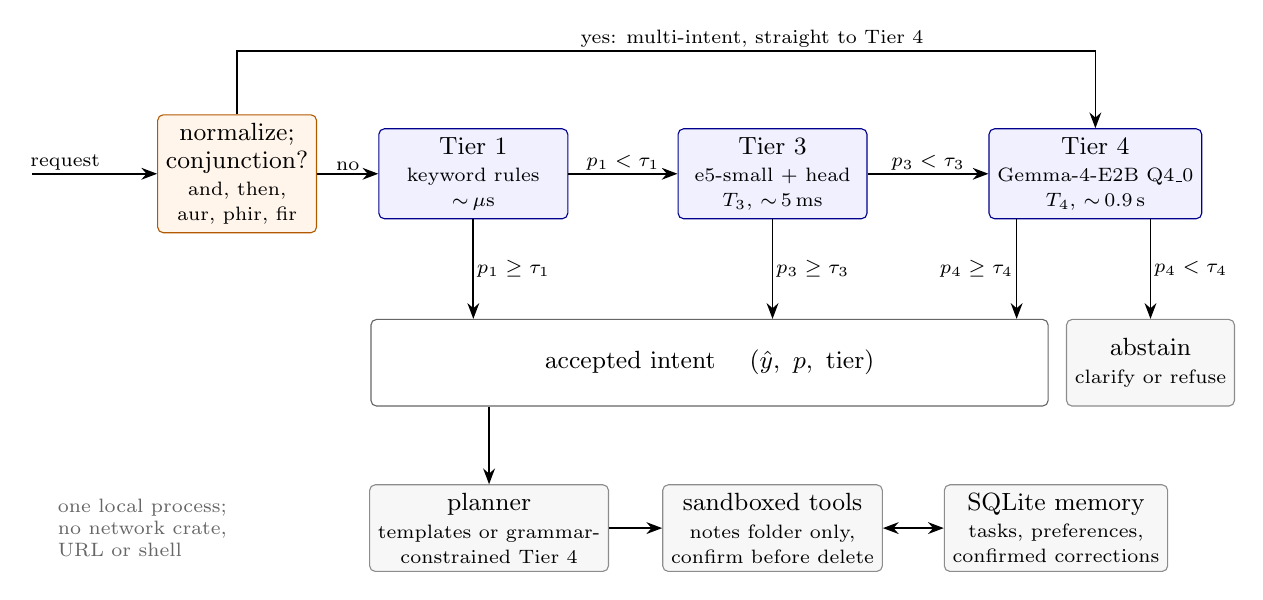
\begin{tikzpicture}[
  font=\small,
  box/.style={draw, rounded corners=2pt, align=center, minimum height=11mm, inner sep=3pt, fill=white},
  tier/.style={box, draw=blue!55!black, fill=blue!6, minimum width=24mm},
  aux/.style={box, draw=black!45, fill=black!3},
  arr/.style={-{Stealth[length=2mm]}, semithick},
  lab/.style={font=\scriptsize, fill=white, inner sep=1pt},
]
\node[box, draw=orange!70!black, fill=orange!8] (sig) at (2.6,0)
  {normalize;\\[-1pt]conjunction?\\[-1pt]\scriptsize and, then,\\[-2pt]\scriptsize aur, phir, fir};
\node[tier] (t1) at (5.6,0) {Tier 1\\[-1pt]\scriptsize keyword rules\\[-2pt]\scriptsize $\sim$\,$\mu$s};
\node[tier] (t3) at (9.4,0) {Tier 3\\[-1pt]\scriptsize e5-small + head\\[-2pt]\scriptsize $T_3$, $\sim$\,5\,ms};
\node[tier] (t4) at (13.5,0) {Tier 4\\[-1pt]\scriptsize Gemma-4-E2B Q4\_0\\[-2pt]\scriptsize $T_4$, $\sim$\,0.9\,s};
\draw[arr] (0,0) node[lab, above right, xshift=-2pt] {request} -- (sig.west);
\draw[arr] (sig) -- node[lab, above] {no} (t1);
\draw[arr] (t1) -- node[lab, above] {$p_1<\tau_1$} (t3);
\draw[arr] (t3) -- node[lab, above] {$p_3<\tau_3$} (t4);
\draw[arr] (sig.north) -- ++(0,0.8) -| node[lab, pos=0.3, above] {yes: multi-intent, straight to Tier 4} (t4.north);
\node[box, minimum width=86mm, draw=black!60] (acc) at (8.6,-2.4) {accepted intent \quad $(\hat y,\ p,\ \text{tier})$};
\node[aux] (abs) at (14.2,-2.4) {abstain\\[-1pt]\scriptsize clarify or refuse};
\draw[arr] (t1.south) -- node[lab, right] {$p_1\ge\tau_1$} (t1.south |- acc.north);
\draw[arr] (t3.south) -- node[lab, right] {$p_3\ge\tau_3$} (t3.south |- acc.north);
\coordinate (a4) at (12.5,0);
\draw[arr] (t4.south -| a4) -- node[lab, left] {$p_4\ge\tau_4$} (a4 |- acc.north);
\draw[arr] (t4.south -| abs.north) -- node[lab, right] {$p_4<\tau_4$} (abs.north);
\node[aux] (plan) at (5.8,-4.5) {planner\\[-1pt]\scriptsize templates or grammar-\\[-2pt]\scriptsize constrained Tier 4};
\node[aux] (tools) at (9.4,-4.5) {sandboxed tools\\[-1pt]\scriptsize notes folder only,\\[-2pt]\scriptsize confirm before delete};
\node[aux] (mem) at (13.0,-4.5) {SQLite memory\\[-1pt]\scriptsize tasks, preferences,\\[-2pt]\scriptsize confirmed corrections};
\draw[arr] (plan.north |- acc.south) -- (plan.north);
\draw[arr] (plan) -- (tools);
\draw[{Stealth[length=2mm]}-{Stealth[length=2mm]}, semithick] (tools) -- (mem);
\node[font=\scriptsize, text=black!60, align=left, anchor=west] at (0.2,-4.5)
  {one local process;\\no network crate,\\URL or shell};
\end{tikzpicture}
\caption{The Kestrel cascade (diagram D1). A request ends at the first tier whose calibrated confidence reaches its
threshold; requests with a conjunction go straight to Tier~4. On CLINC150 the cascade is Tier~3 $\to$ Tier~4. Latencies
are orders of magnitude on the test machine (Table~\ref{tab:r1}). The planner, tools and memory serve the assistant;
the evaluation scores the routing decision.}
\label{fig:arch}
\end{figure}

% ---------------------------------------------------------------------------------------------------------------
\section{Experimental Setup}\label{sec:setup}

\paragraph{Hardware and software.} One laptop: AMD Ryzen~5 5500U (6 cores, 12 threads), 14.95~GiB RAM, Fedora~44
(Linux 7.2.6), Rust 1.99.0, Python 3.14.7, llama.cpp commit \texttt{26394b4e} through \texttt{llama-cpp-2} 0.1.157.
Models are loaded without memory mapping, so peak RSS (\texttt{VmHWM}) is the real footprint.

\paragraph{Datasets.} \emph{CLINC150}~\citep{larson2019clinc} (full version): train 15\,000, calibration 1\,500,
validation 1\,700 (with 200 OOS) and the official test set, $n=\kv{clinc.n}$ with 1\,000 OOS requests. The 100 official
OOS training items join validation, and the 14 test items whose text also occurs in another split are kept, with a
sensitivity analysis that drops them. \emph{Kestrel-Intents-v0} is a synthetic set of assistant requests in English and
Hinglish (romanized Hindi--English), drafted with an AI assistant from templates and reviewed by the author: train 604,
calibration 100, validation 128, test $n=\kv{intents.n}$ (126 per language, \kv{intents.clusters} template families).
It is split by template family, its test OOS requests come from unseen domains, and its compound requests occur only
in validation and test. It is labelled synthetic in every table.

\paragraph{Pre-registration.} Hypotheses, systems, scoring, the measurement protocol, invalidation rules and the
analysis were written in a pre-registration and frozen (git tag \texttt{exp-E1-frozen}) before any test item was read.
One later clarification, which fixed the datasets of three secondary hypotheses, is disclosed
(Section~\ref{sec:threats}). The margin $\delta=\kv{delta}$ is twice the seed-to-seed standard deviation of the tuned
SLM's accuracy in a five-seed pilot on validation data; it exceeds the provisional smallest effect of interest, 0.02.

\paragraph{Measurement protocol.} AC power, the \texttt{performance} governor, turbo boost off, six threads pinned
one per physical core, background services stopped, and at least five minutes of cooldown below 50\,\textdegree C
before each session. One process loads every model once; the systems run in rotated order per item and repetition
after five warm-up requests each. Per item, latency is the median of 5 timed repetitions of the end-to-end wall time
on a monotonic clock (Kestrel-Intents-v0: all items; CLINC150: a fixed, seeded 20\% subset of
\kv{clinc.timed} items, with one timed run on the rest, so latency statistics use the subset and accuracy all items).
Runs are cut into chunks of about one hour, each with its own pre-checks. Five pre-declared rules invalidate a chunk
(lost AC power or boost on; background load above 10\%; a frequency deviation above 10\%; a temperature above
95\,\textdegree C; a crash or model-hash mismatch). Every test run was valid at the first attempt. Model loading is
excluded from latency. Energy was not measured, because the only counter (RAPL) is root-only on this machine.

\paragraph{Statistics.} Paired bootstrap with 10\,000 resamples (seed 0)~\citep{efron1993bootstrap} gives 95\% CIs. On
Kestrel-Intents-v0 the bootstrap resamples template families, since items of one family are not
independent~\citep{field2007cluster}. H1 is an intersection--union test~\citep{berger1982iut}: the lower CI bound of
$\Delta$accuracy above $-\delta$ \emph{and} the upper CI bound of $\Delta$latency below 0. The 13 secondary members get
one p-value each on the two-sided scale (bootstrap for margins and non-0/1 statistics, exact
McNemar~\citep{mcnemar1947} for paired correctness, Wilcoxon signed-rank for latency and paired runs) and are adjusted
together by Holm's method~\citep{holm1979}. Outcomes are \emph{supported} (adjusted $p<0.05$ in the hypothesized
direction), \emph{not supported} (the CI wholly on the wrong side) or \emph{inconclusive}. We follow common guidance on
significance testing and reporting in NLP~\citep{dror2018hitchhiker,dodge2019showyourwork}.

% ---------------------------------------------------------------------------------------------------------------
\section{Baselines}\label{sec:baselines}

All systems share the same models, prompt templates, grammar and thread count, and each receives the same tuning
effort: one abstention threshold chosen on validation.
\textbf{R0} always uses the SLM (Tier~4) and abstains below a tuned threshold on its calibrated confidence;
\textbf{R0 untuned} always answers. \textbf{R1} uses the encoder head alone with a tuned threshold.
\textbf{R2} is the cascade on raw confidences with one shared threshold, and \textbf{R2c} the same with calibrated
confidences (used for RQ2). \textbf{R3} is the calibrated cascade with per-tier thresholds at the operating point of
Eq.~\eqref{eq:op}. \textbf{R-rand} escalates at random with R3's per-tier escalation rates, so its expected cost
matches R3's; its accuracy is an expectation over at least 1\,000 seeds. For RQ5 the baselines are naive fine-tuning,
online EWC~\citep{kirkpatrick2017ewc} and replay, with joint training as an upper bound and the stage-0 head as a lower
bound, all with the same hyperparameter budget (12 configurations per method).

% ---------------------------------------------------------------------------------------------------------------
\section{Evaluation Metrics}\label{sec:metrics}

\emph{Accuracy} uses the scoring rule of Section~\ref{sec:problem}; \emph{macro-F1} averages over gold classes, counting
an abstention as the OOS label; \emph{coverage} is the share of requests answered. \emph{Selective risk} at coverage
0.80 is the error rate among answered requests at the smallest coverage $\ge 0.80$. \emph{AURC} is the area under the
risk--coverage curve on a 20-point grid. \emph{ECE} uses 15 equal-width, right-closed bins. \emph{Latency} is reported
as the mean, median and nearest-rank p95 over per-item medians; \emph{peak RSS} is \texttt{VmHWM} of a process that
loads only one system's models. For RQ5, with $R_{i,j}$ the accuracy on stage $j$ after training stage $i$ of $S$
stages, we report average final accuracy, average forgetting~\citep{chaudhry2018riemannian} and backward
transfer~\citep{lopezpaz2017gem}.

% ---------------------------------------------------------------------------------------------------------------
\section{Results}\label{sec:results}

\begin{table}[t]
\centering\small
\caption{Routing policies on the test sets (E1; Table R1 of the protocol). Accuracy counts abstention on an in-scope item as an error.
Latency is per request on a warm process, model loading excluded; ``Tier 4'' is the share of requests that reached the
SLM. Kestrel-Intents-v0 is synthetic.}
\label{tab:r1}
\textbf{CLINC150} ($n=\kv{clinc.n}$; latency on \kv{clinc.timed} timed items)\\[2pt]
\resizebox{\textwidth}{!}{% Generated by experiments/analysis/paper_assets.py.
\begin{tabular}{lrrrrrrrr}
\toprule
System & Accuracy & Macro-F1 & Coverage & Mean ms & Median ms & p95 ms & Peak RSS MiB & Tier 4 \\
\midrule
R0 & 0.827 & 0.870 & 0.875 & 863 & 865.0 & 1292 & 3491 & 100\% \\
R0 untuned & 0.773 & 0.850 & 1.000 & 863 & 865.0 & 1292 & 3491 & 100\% \\
R1 & 0.893 & 0.925 & 0.811 & 6 & 5.4 & 8 & 278 & 0\% \\
R3 & 0.874 & 0.914 & 0.890 & 146 & 5.6 & 931 & 3773 & 17\% \\
\bottomrule
\end{tabular}
}\\[8pt]
\textbf{Kestrel-Intents-v0, synthetic} ($n=\kv{intents.n}$, all timed)\\[2pt]
\resizebox{\textwidth}{!}{% Generated by experiments/analysis/paper_assets.py.
\begin{tabular}{lrrrrrrrr}
\toprule
System & Accuracy & Macro-F1 & Coverage & Mean ms & Median ms & p95 ms & Peak RSS MiB & Tier 4 \\
\midrule
R0 & 1.000 & 1.000 & 1.000 & 689 & 669.5 & 916 & 3367 & 100\% \\
R0 untuned & 1.000 & 1.000 & 1.000 & 689 & 669.5 & 916 & 3367 & 100\% \\
R1 & 0.702 & 0.860 & 1.000 & 6 & 5.6 & 9 & 276 & 0\% \\
R3 & 0.968 & 0.989 & 1.000 & 382 & 521.7 & 917 & 3638 & 54\% \\
\bottomrule
\end{tabular}
}
\end{table}

\begin{figure}[t]
\centering
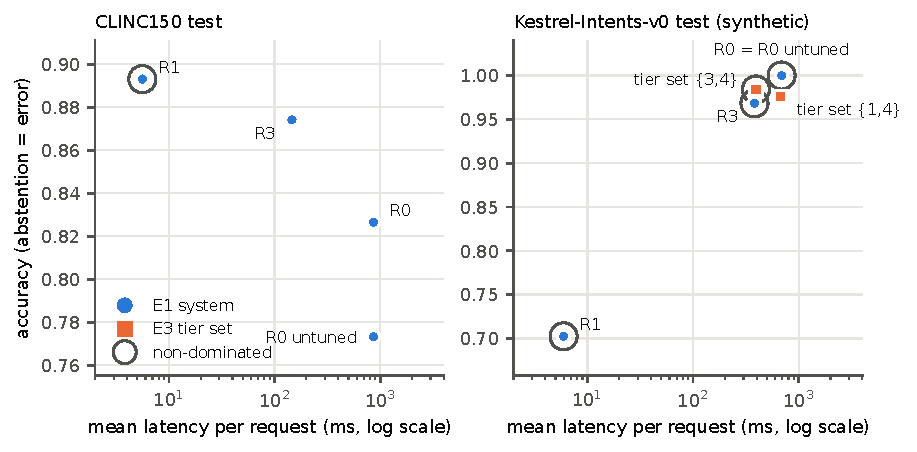
\includegraphics[width=\textwidth]{figures/frontier.pdf}
\caption{Accuracy against mean latency on the test sets: the E1 systems and the extra tier sets of E3. Ringed points
are not dominated (no other point is both at least as accurate and at least as fast). On CLINC150 the encoder alone (R1)
dominates the cascade (R3).}
\label{fig:frontier}
\end{figure}

\subsection{RQ1: the cascade against the single models (E1)}

\paragraph{H1, primary (CLINC150): supported.} At its validation-chosen operating point the cascade answered
\kv{clinc.r3.tfour} of requests with the SLM, reached accuracy \kv{clinc.r3.acc} against \kv{clinc.r0.acc} for
the tuned SLM, $\Delta$accuracy \kv{clinc.h1.dacc} (95\% CI \kv{clinc.h1.dacc.ci}), with $\Delta$mean latency
\kv{clinc.h1.dlat}\ms\ (CI \kv{clinc.h1.dlat.ci}); see Table~\ref{tab:r1}. Both parts of the intersection--union test
hold, and the result is \kv{clinc.h1.outcome}. Dropping the 14 test items that also occur in other splits
($n=\kv{clinc.done.n}$) leaves the accuracy CI at \kv{clinc.done.dacc.ci}. The median latency of requests that the
cascade answered below Tier~4 was \kv{clinc.rho.rthree}\ms, against \kv{clinc.r0.median}\ms\ for the SLM. The p95
latency, \kv{clinc.r3.p95}\ms, is set by the requests that do reach Tier~4. The cascade does not save memory: it keeps
the encoder loaded next to the SLM, and its peak RSS was \kv{clinc.r3.rss}~MiB against \kv{clinc.r0.rss}~MiB.

\paragraph{H1b: better than random escalation at the same cost (supported on both datasets).} R-rand, which escalates
as often as R3 at random, reached \kv{clinc.rrand.acc} on CLINC150 (R3 $-$ R-rand: \kv{clinc.h1b.dacc}, CI
\kv{clinc.h1b.dacc.ci}) and \kv{intents.rrand.acc} on Kestrel-Intents-v0 (\kv{intents.h1b.dacc}, CI
\kv{intents.h1b.dacc.ci}). The confidence signal, not just the escalation rate, is what earns the accuracy.

\paragraph{H1c: against the encoder alone (CLINC150 inconclusive, Kestrel-Intents-v0 supported).} On CLINC150 the
encoder alone was more accurate than the cascade (\kv{clinc.r1.acc} vs \kv{clinc.r3.acc}; $\Delta$
\kv{clinc.h1c.dacc}, CI \kv{clinc.h1c.dacc.ci}) and faster (mean \kv{clinc.r1.mean} vs \kv{clinc.r3.mean}\ms), so
R1 dominates R3 on the test frontier
(Figure~\ref{fig:frontier}). The CI's lower bound lies just inside the margin (unadjusted $p=\kv{fam.H1c-CLINC150.p}$),
but not after Holm adjustment ($p=\kv{fam.H1c-CLINC150.holm}$). On Kestrel-Intents-v0 the encoder alone was far weaker
(\kv{intents.r1.acc}) and the cascade gained \kv{intents.h1c.dacc} (CI \kv{intents.h1c.dacc.ci}). Section~\ref{sec:discussion}
explains the CLINC150 result.

\paragraph{H1 on Kestrel-Intents-v0: inconclusive.} Here the SLM was perfect (\kv{intents.r0.acc}). The cascade
was faster ($\Delta$mean latency \kv{intents.h1.dlat}\ms, CI \kv{intents.h1.dlat.ci}) but less accurate
($\Delta$accuracy \kv{intents.h1.dacc}, CI \kv{intents.h1.dacc.ci}). The CI crosses $-\delta$, so non-inferiority is not shown, and its upper bound is below 0.

\paragraph{RQ7, H7a: Hinglish (inconclusive).} On Hinglish requests the cascade stayed close to the SLM
($\Delta$ \kv{intents.hi.dacc}, CI \kv{intents.hi.dacc.ci}; unadjusted $p=\kv{fam.H7a.p}$, Holm
$p=\kv{fam.H7a.holm}$); on English it lost more ($\Delta$ \kv{intents.en.dacc}, CI \kv{intents.en.dacc.ci}; reported,
not tested). Hinglish requests reached the SLM more often (\kv{intents.hi.tfour} vs \kv{intents.en.tfour}), so they cost
more (mean \kv{intents.hi.rthree.mean}\ms\ vs \kv{intents.en.rthree.mean}\ms); this is descriptive, as pre-registered.

\subsection{RQ2: calibration (E2)}

\begin{table}[t]
\centering\small
\caption{Per-tier calibration on test, single-intent in-scope items (E2; Table R2). $T$ is fitted on the calibration
split; risk is at coverage 0.80 within the tier.}
\label{tab:r2}
% Generated by experiments/analysis/paper_assets.py.
\begin{tabular}{llrrrrrrr}
\toprule
Data & Tier & n & Acc. & $T$ & ECE raw & ECE cal. & Risk@0.8 raw & Risk@0.8 cal. \\
\midrule
CLINC150 & Tier 3 & 4500 & 0.959 & 0.666 & 0.0553 & 0.0083 & 0.0058 & 0.0058 \\
CLINC150 & Tier 4 & 4500 & 0.904 & 1.263 & 0.0489 & 0.0216 & 0.0297 & 0.0294 \\
Intents-v0 & Tier 3 & 204 & 0.868 & 0.688 & 0.0590 & 0.0557 & 0.0671 & 0.0671 \\
Intents-v0 & Tier 4 & 204 & 1.000 & 0.847 & 0.0097 & 0.0058 & 0.0000 & 0.0000 \\
\bottomrule
\end{tabular}

\end{table}

\begin{figure}[t]
\centering
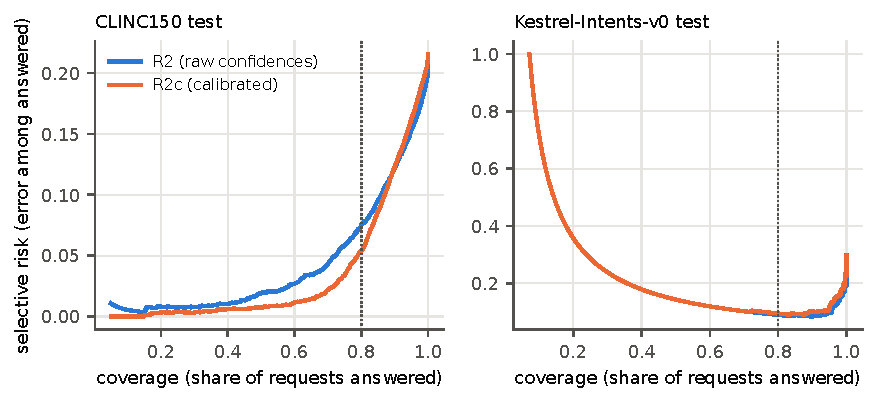
\includegraphics[width=\textwidth]{figures/riskcov.pdf}
\caption{Risk--coverage curves of the cascade with one shared threshold on raw (R2) and calibrated (R2c) confidences,
test sets. The dotted line marks coverage 0.80, where H2 is tested.}
\label{fig:riskcov}
\end{figure}

Temperature scaling reduced the encoder head's ECE on CLINC150 from \kv{clinc.tthree.ece.before} to
\kv{clinc.tthree.ece.after} ($T_3=\kv{clinc.tthree.T}$, so the raw head was under-confident) and Tier~4's from
\kv{clinc.tfourcal.ece.before} to \kv{clinc.tfourcal.ece.after} (Table~\ref{tab:r2}). For Tier~3 a temperature
is monotone and cannot reorder requests; for Tier~4, whose confidence multiplies several decoding steps, it can, but
little. Per-tier selective risk therefore barely moves, and calibration acts by making the tiers' confidences comparable
under one shared threshold.

\paragraph{H2 (CLINC150 supported, Kestrel-Intents-v0 inconclusive).} On CLINC150, calibration lowered selective risk
at coverage 0.80 from \kv{clinc.risk.rtwo} to \kv{clinc.risk.rtwoc} ($\Delta$ \kv{clinc.risk.diff}, CI
\kv{clinc.risk.diff.ci}) and AURC from \kv{clinc.aurc.rtwo} to \kv{clinc.aurc.rtwoc} (Figure~\ref{fig:riskcov}). On
Kestrel-Intents-v0 it did not replicate: risk \kv{intents.risk.rtwo} vs \kv{intents.risk.rtwoc} ($\Delta$
\kv{intents.risk.diff}, CI \kv{intents.risk.diff.ci}), and AURC was slightly worse with calibration ($\Delta$
\kv{intents.aurc.diff}, CI \kv{intents.aurc.diff.ci}). The Tier-3 temperature fitted on 100 synthetic calibration items
hardly changed that tier's ECE (\kv{intents.tthree.ece.before} to \kv{intents.tthree.ece.after}).

\paragraph{H7b: calibration by language (inconclusive).} With one temperature for both languages, Tier~3's ECE was
\kv{intents.hsevenb.en} on English and \kv{intents.hsevenb.hi} on Hinglish (gap \kv{intents.hsevenb.gap}, CI
\kv{intents.hsevenb.gap.ci}; unadjusted $p=\kv{fam.H7b.p}$).

\subsection{RQ5: forgetting in the trainable head (E5)}

\begin{table}[t]
\centering\small
\caption{Class-incremental updates of the Tier-3 head on CLINC150 (E5; Table R6): 10 domains in 5 stages of 2, mean
$\pm$ SD over 15 runs (3 domain orders $\times$ 5 seeds), configurations selected on validation.}
\label{tab:r6}
% Generated by experiments/analysis/paper_assets.py.
\begin{tabular}{lrrrrr}
\toprule
Method & Avg. accuracy & Avg. forgetting & BWT & Update s & Buffer MB \\
\midrule
naive & 0.188 $\pm$ 0.005 & 0.947 $\pm$ 0.006 & -0.947 & 3.6 & 0.0 \\
replay & 0.918 $\pm$ 0.004 & -0.002 $\pm$ 0.005 & +0.006 & 7.0 & 9.3 \\
ewc & 0.183 $\pm$ 0.004 & 0.932 $\pm$ 0.007 & -0.932 & 6.0 & 0.0 \\
joint & 0.928 $\pm$ 0.003 & 0.012 $\pm$ 0.003 & -0.011 & 9.5 & 0.0 \\
stage0 & 0.188 $\pm$ 0.005 & 0.000 $\pm$ 0.000 & +0.000 & 0.8 & 0.0 \\
\bottomrule
\end{tabular}

\end{table}

\begin{figure}[t]
\centering
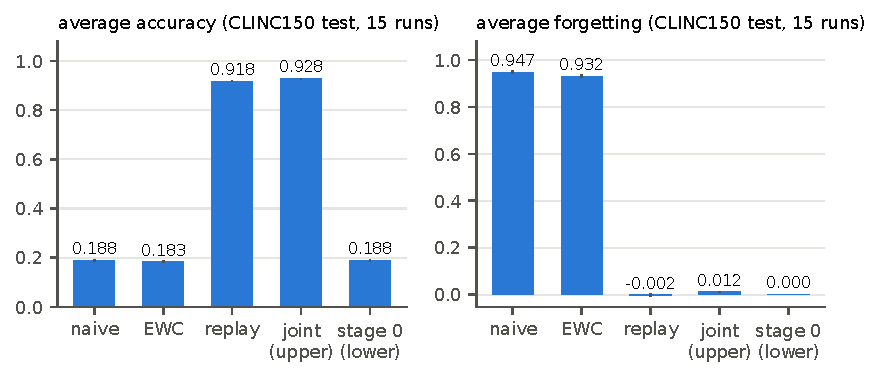
\includegraphics[width=0.9\textwidth]{figures/e5.pdf}
\caption{Average accuracy and forgetting of each update method (CLINC150 test, 15 runs; bars show the mean, error bars
the SD).}
\label{fig:e5}
\end{figure}

Updating the head on each new stage alone (naive) forgot almost everything learned earlier: average forgetting
\kv{e5.naive.forget} and average accuracy \kv{e5.naive.acc}, no better than never updating (stage 0,
\kv{e5.stage0.acc}). Replay of 50 stored items per earlier class removed the forgetting
(\kv{e5.replay.forget}; accuracy \kv{e5.replay.acc}, close to joint training's \kv{e5.joint.acc}).
\textbf{H5 is supported}: replay minus naive forgetting \kv{e5.h5.diff} (CI \kv{e5.h5.diff.ci}; Wilcoxon over the 15
paired runs, $p=\kv{e5.h5.p}$). EWC changed forgetting by only \kv{e5.ewc.diff} relative to naive (reported, outside
the family): the empirical Fisher information was small, and SGD's stability bound capped the penalty weight. The price
of replay is its buffer, which stores half of every earlier class's training items (Table~\ref{tab:r6}).

\subsection{All pre-registered hypotheses}

\begin{table}[t]
\centering\small
\caption{The secondary family (Holm, 13 members). H4 and H6 have not run; they enter with $p=1$ until their amendment,
so every adjustment is interim: an interim ``supported'' is final, and an interim ``inconclusive'' may still change.
H1 on CLINC150 is the primary and is tested alone.}
\label{tab:family}
% Generated by experiments/analysis/paper_assets.py.
\begin{tabular}{lllll}
\toprule
Hypothesis & $p$ & Holm $p$ & Outcome & Source \\
\midrule
H1 Intents-v0 & $1$ & $1$ & inconclusive (interim) & E1 Intents-v0 \\
H1b CLINC150 & $<10^{-4}$ & $<10^{-4}$ & supported & E1 CLINC150 \\
H1b Intents-v0 & $2.0\times 10^{-4}$ & $0.002$ & supported & E1 Intents-v0 \\
H1c CLINC150 & $0.045$ & $0.27$ & inconclusive (interim) & E1 CLINC150 \\
H1c Intents-v0 & $<10^{-4}$ & $<10^{-4}$ & supported & E1 Intents-v0 \\
H2 CLINC150 & $<10^{-4}$ & $<10^{-4}$ & supported & E2 CLINC150 \\
H2 Intents-v0 & $1$ & $1$ & inconclusive (interim) & E2 Intents-v0 \\
H3 & $0.006$ & $0.045$ & supported & E3 Intents-v0 \\
H4 & $\text{pending}$ & $\text{pending}$ & pending & --- \\
H5 & $6.1\times 10^{-5}$ & $6.1\times 10^{-4}$ & supported & E5 CLINC150 \\
H6 & $\text{pending}$ & $\text{pending}$ & pending & --- \\
H7a & $0.036$ & $0.25$ & inconclusive (interim) & E1 Intents-v0 hi-en \\
H7b & $0.06$ & $0.30$ & inconclusive (interim) & E2 Intents-v0 \\
\bottomrule
\end{tabular}

\end{table}

Table~\ref{tab:family} lists every member: \kv{fam.supported} of 13 are supported, none is not supported, five are
inconclusive and two are pending.

% ---------------------------------------------------------------------------------------------------------------
\section{Ablation Studies}\label{sec:ablation}

\begin{table}[t]
\centering\small
\caption{Tier ablation on test (E3; Table R3); each set is tuned on validation by the same rule. On CLINC150 the rules
cannot answer, so only $\{4\}$ and $\{3,4\}$ apply.}
\label{tab:r3}
% Generated by experiments/analysis/paper_assets.py.
\begin{tabular}{llrrrl}
\toprule
Data & Tier set & Accuracy & Mean ms & p95 ms & Ended at Tier 1 / 3 / 4 \\
\midrule
CLINC150 & \{4\} & 0.827 & 863 & 1292 & 0.00 / 0.00 / 1.00 \\
CLINC150 & \{3,4\} & 0.874 & 146 & 933 & 0.00 / 0.83 / 0.17 \\
Intents-v0 & \{4\} & 1.000 & 689 & 916 & 0.00 / 0.00 / 1.00 \\
Intents-v0 & \{1,4\} & 0.976 & 670 & 916 & 0.02 / 0.00 / 0.98 \\
Intents-v0 & \{3,4\} & 0.984 & 394 & 912 & 0.00 / 0.45 / 0.55 \\
Intents-v0 & \{1,3,4\} & 0.968 & 382 & 912 & 0.02 / 0.44 / 0.54 \\
\bottomrule
\end{tabular}

\end{table}

\paragraph{H3: adding the encoder to rules + SLM (supported).} On Kestrel-Intents-v0, adding Tier~3 to
\tierset{1,4} kept accuracy within the margin ($\Delta$ \kv{intents.hthree.dacc}, CI \kv{intents.hthree.dacc.ci})
and lowered mean cost ($\Delta$ \kv{intents.hthree.dcost}\ms, CI \kv{intents.hthree.dcost.ci}), Holm
$p=\kv{fam.H3.holm}$ (Table~\ref{tab:r3}). On CLINC150, \tierset{3,4} against \tierset{4} is the H1 comparison
($\Delta$ \kv{clinc.hthree.dacc}, \kv{clinc.hthree.dcost}\ms). Tier~2 was not built, so H3's clause about it is
untested.

\paragraph{The rules cost accuracy on test.} \tierset{1,4} was less accurate than \tierset{4} (\kv{intents.set14.acc}
vs \kv{intents.set4.acc}) for a small saving (\kv{intents.set14.cost} vs \kv{intents.set4.cost}\ms), and the best
point on the Kestrel test frontier was \tierset{3,4} (\kv{intents.set34.acc} at \kv{intents.set34.cost}\ms). The
failure analysis (Section~\ref{sec:discussion}) shows why.

\paragraph{Calibration.} RQ2 is the calibration ablation (Section~\ref{sec:results}). On the validation
accuracy--cost frontier, temperature scaling did not move the cascade's points (a development finding): a per-tier
threshold absorbs a monotone temperature, and on the frontier Tier~4 always answers. Its effect is on abstention quality
under a shared threshold.

% ---------------------------------------------------------------------------------------------------------------
\section{Discussion}\label{sec:discussion}

\paragraph{Each single model wins on one dataset; the cascade wins on neither.} The SLM alone is best on
Kestrel-Intents-v0 and the encoder alone on CLINC150 (Figure~\ref{fig:frontier}). The cascade sits between them: it
is much better than the weaker single model on each dataset (\kv{clinc.h1.dacc} over the SLM on CLINC150,
\kv{intents.h1c.dacc} over the encoder on Kestrel-Intents-v0) and much cheaper than the SLM. Its operating point was
chosen to match the better single model on validation, and it did there, but not on test. The honest summary is a
hedge: a deployment that cannot know in advance which model suits its traffic loses little with the cascade, but a
deployment whose traffic resembles CLINC150 would do better with the encoder alone.

\paragraph{Why the cascade lost to the encoder on CLINC150 (exploratory).} The cascade made \kv{err.clinc.errors}
errors on CLINC150, and \kv{err.clinc.ooserrors} of them (\kv{err.clinc.oosshare}) were out-of-scope requests answered
with an in-scope intent. The operating point accepts Tier~3 at confidence $\ge\kv{err.clinc.tau.rthree}$, the cheapest
point that met the floor on validation, while R1 abstains below \kv{err.clinc.tau.rone}; \kv{err.clinc.band}
out-of-scope test requests fall between the two, and the cascade answers them. OOS requests were
\kv{err.clinc.oos.val} of validation but \kv{err.clinc.oos.test} of test, so a threshold chosen for cost on validation
under-weights them. This is a shift in the OOS rate, not a calibration failure (Tier~3's test ECE after scaling is
\kv{clinc.tthree.ece.after}), and it matches the known weakness of confidence-based deferral under
shift~\citep{jitkrittum2023deferral}. Remedies to test in a new, pre-registered version: a reject band at Tier~3, an OOS
detector before Tier~3, or a validation set with the deployment's OOS share.

\paragraph{Why the rules hurt on Kestrel-Intents-v0 (exploratory).} Of the cascade's \kv{err.intents.errors} errors,
\kv{err.intents.compound} were compound requests joined by \emph{also} or \emph{, now}, which the conjunction signal
does not know, so a single-intent rule accepted them. All \kv{err.intents.valcompounds} validation compounds contained
a signal word, so tuning could not see the gap. A wider signal is a post-hoc change and would be evaluated as such.

\paragraph{Practical guidance.} (1) Measure the OOS share of real traffic and choose the operating point on data that
matches it. (2) Report the encoder alone with a tuned threshold as a baseline: it is cheap and, on CLINC150, the system
to beat. (3) A cascade saves latency, not memory: keeping a 4-bit SLM resident costs about \kv{clinc.r0.rss}~MiB
whether or not most requests use it. (4) Calibrate when one threshold compares confidences across tiers; with per-tier
thresholds the frontier does not change.

% ---------------------------------------------------------------------------------------------------------------
\section{Threats to Validity}\label{sec:threats}

\paragraph{Internal.} Thresholds and temperatures were tuned only on calibration and validation data, and the
configurations were frozen and tagged before the test sets were read. After the freeze, one clarification fixed which
datasets enter the family for H1b, H1c and H2; by then E5's and Kestrel-Intents-v0's E2 results had been seen, and both
datasets were kept in the family. Thermal and background effects are controlled by the pinned protocol and the five
invalidation rules, and no test chunk was invalidated. Systems were interleaved per item, so slow drift affects them
alike. The failure analysis was done after the results were read and is labelled exploratory.

\paragraph{External.} One machine, one SLM and one encoder; turbo boost was off, so absolute latencies are conservative
and other CPUs, GPUs or NPUs may change the ratios. Kestrel-Intents-v0 is synthetic, small, and drafted with an AI
assistant, and its labels were frozen before a second annotator measured agreement. Hinglish appears only in this set.

\paragraph{Construct.} Counting abstention as an error on in-scope items, but as correct on OOS items, rewards
cautious systems on CLINC150, with its high OOS share. We report coverage and macro-F1 next to accuracy for this reason.
Latency excludes model loading (tens of seconds) and is measured on a warm, single-user process. Energy was not
measured.

\paragraph{Contamination.} CLINC150 has been public since 2019 and may be in the SLM's pre-training data. This cannot
be ruled out, but it would favour R0, against which the cascade was compared.

\paragraph{Statistical.} The family's adjusted p-values are interim until H4 and H6 run. The margin $\delta$ was frozen
before the mentor confirmed the smallest effect of interest; a larger one would turn H1 into a sensitivity analysis.

% ---------------------------------------------------------------------------------------------------------------
\section{Limitations}\label{sec:limits}

We did not test: other hardware, other SLMs or encoders, or quantization levels (E6, H6, pending); personalization from
corrections (E4, H4, pending, waiting on the review of its synthetic personas); a Tier-2 distilled model; a learned
deferral gate; energy; or any public code-mixed benchmark. The per-language intervals are wide with 126 items per
language. ``No network'' is shown for the tested scenarios only; it is not a formal privacy guarantee, nothing confines
the process at kernel level, and swap, crash dumps and backups are not covered. The heads are trained in Python and
not stored in git, and whether retraining gives the same bytes on another platform has not been checked.

% ---------------------------------------------------------------------------------------------------------------
\section{Ethical Considerations}\label{sec:ethics}

\paragraph{Local data handling.} All inference runs on the user's machine. A privacy check
(\kv{priv.pass}/\kv{priv.total} passing) shows no network crates in the dependency tree, no URL and no shell in the
runtime code, zero \texttt{connect()} calls under a network namespace in the tested scenarios (with a deliberate
connection as a positive control), no files opened outside the allowed roots, and a planted canary absent from
telemetry and gone from the database after deletion.

\paragraph{Consent for learning.} Kestrel asks before it stores a correction or a learned alias, and the user can list,
export, delete or purge the memory. The replay buffer that prevents forgetting (RQ5) keeps users'
own request texts; storing or training on user text carries a memorization risk~\citep{carlini2021extracting}, and
formal guarantees such as differential privacy~\citep{abadi2016dpsgd} were not applied.

\paragraph{Tools.} Tools are allow-listed, confined to the notes folder by a path sandbox that rejects traversal and
symbolic links, and destructive actions ask first.

\paragraph{Synthetic data and AI assistance.} Kestrel-Intents-v0 and the draft persona and task sets are synthetic,
were drafted with an AI coding assistant, and describe no real person. The code and analysis scripts were also written
with that assistant under the author's review; the pre-registration, design decisions and their rationale are the
author's and are logged with dates.

% ---------------------------------------------------------------------------------------------------------------
\section{Reproducibility}\label{sec:repro}

\begin{sloppypar}
The repository pins the Rust toolchain and crates (\texttt{Cargo.lock}), Python packages (\texttt{requirements.lock}),
every model by repository, revision and SHA-256 (the encoder GGUF is converted locally by a pinned script), and the
datasets by commit and SHA-256. Every run writes a manifest with the environment, hashes, checks and a validity flag.
One command (\texttt{python experiments/repro.py -{}-rerun-e5}) clones the committed state into a scratch directory,
regenerates every analysis from the raw logs and compares the outputs. At commit \kv{repro.head},
\kv{repro.identical} of 11 outputs were byte-identical, and the E5 rerun gave equal numbers. This paper's numbers,
tables and figures are generated from the same logs (\texttt{experiments/analysis/paper\_assets.py}). A reproduction
on a second machine is planned and has not been done. Licences: CLINC150 CC BY 3.0, Gemma-4 Apache-2.0,
multilingual-e5-small MIT, Kestrel's code MIT or Apache-2.0.
\end{sloppypar}

% ---------------------------------------------------------------------------------------------------------------
\section{Conclusion}\label{sec:conclusion}

On one laptop CPU and under a frozen protocol, a calibrated rules--encoder--SLM cascade was as accurate as always using
the SLM, and faster, on CLINC150 ($\Delta$accuracy \kv{clinc.h1.dacc}, $\Delta$mean latency
\kv{clinc.h1.dlat}\ms\ per request; RQ1, H1 supported), and its confidence signal beat random escalation at equal cost on both datasets (H1b).
Calibration lowered selective risk on CLINC150 but not on the synthetic set (RQ2). Adding the encoder to rules and SLM
changed mean cost by \kv{intents.hthree.dcost}\ms\ per request with accuracy within the margin (RQ3), and replay removed the head's forgetting
(RQ5). What was \emph{not} supported matters as much. The cascade did not beat the encoder alone on CLINC150, where the
encoder dominated it, or the SLM alone on the synthetic set. The cascade's advantage over the single models therefore
depends on traffic, notably on the out-of-scope share. Its Hinglish behaviour (RQ7) remains inconclusive, and
personalization and quantization are still to run.

\bibliographystyle{plainnat}
\bibliography{references}

\end{document}
